
	
%%%%%%%%%%%%%%%%%%%%%%% file typeinst.tex %%%%%%%%%%%%%%%%%%%%%%%%%
%
% This is the LaTeX source for the instructions to authors using
% the LaTeX document class 'llncs.cls' for contributions to
% the Lecture Notes in Computer Sciences series.
% http://www.springer.com/lncs       Springer Heidelberg 2006/05/04
%
% It may be used as a template for your own input - copy it
% to a new file with a new name and use it as the basis
% for your article.
%
% NB: the document class 'llncs' has its own and detailed documentation, see
% ftp://ftp.springer.de/data/pubftp/pub/tex/latex/llncs/latex2e/llncsdoc.pdf
%
%%%%%%%%%%%%%%%%%%%%%%%%%%%%%%%%%%%%%%%%%%%%%%%%%%%%%%%%%%%%%%%%%%%


\documentclass[runningheads,a4paper]{llncs}

\usepackage{amssymb}
\usepackage{amsmath}
\newcommand\numberthis{\addtocounter{equation}{1}\tag{\theequation}}
\setcounter{tocdepth}{3}
\usepackage{graphicx}
\usepackage{rotfloat}
\usepackage{enumitem}
\usepackage{multicol}
\usepackage{multirow}
\usepackage{hyperref}
\usepackage{url}
\usepackage{sectsty}
\usepackage{tabularx}
% \usepackage[section]{placeins}
\usepackage{titlesec}
\newcolumntype{C}{>{\centering\arraybackslash}X}

\sectionfont{\Large}
\subsectionfont{\large}
\renewcommand{\labelitemi}{$\bullet$}

\setlength{\floatsep}{5pt plus 2pt minus 2pt}
\setlength{\abovecaptionskip}{0pt}
\setlength{\belowcaptionskip}{-15pt}

\urldef{\mailsa}\path|{andreas.boltres}@student.kit.edu|    
\newcommand{\keywords}[1]{\par\addvspace\baselineskip
\noindent\keywordname\enspace\ignorespaces#1}

\begin{document}

\hypersetup{
	pdftitle={gym-autokey: RL for Rule-Based Deductive Program Verification in Ke\kern-.1em{Y}},
	pdfauthor={Andreas Boltres}
}

\mainmatter  % start of an individual contribution

% first the title is needed
\title{gym-autokey: RL for Rule-Based Deductive Program Verification in Ke\kern-.1em{Y}}

% a short form should be given in case it is too long for the running head
\titlerunning{gym-autokey: RL for Rule-Based Deductive Program Verification in Ke\kern-.1em{Y}}

% the name(s) of the author(s) follow(s) next
%
% NB: Chinese authors should write their first names(s) in front of
% their surnames. This ensures that the names appear correctly in
% the running heads and the author index.
%
\author{Andreas Boltres}
%
\authorrunning{gym-autokey: RL for Rule-Based Deductive Program Verification in Ke\kern-.1em{Y}}
% (feature abused for this document to repeat the title also on left hand pages)

\institute{Karlsruhe Institute of Technology\\
\url{https://www.kit.edu}}

\maketitle

% ==================================================================================================

\section*{Introduction}

\subsection*{Formal Verification}

\textit{Formal Verification} (FV) is the systematic process of proving or disproving the correctness of an artifact such as an algorithm or a software specification, using formal methods. These formal methods used are mathematically founded, e.g. logic calculi or deduction techniques.

FV applied to the specification of software/code is called \textit{Program-} or \textit{Software Verification} (SV). If the specification of a piece of code can be formally verified, it is guaranteed that the code's behaviour conforms to its specification, which can be a crucial quality aspect regarding performance, security and safety.

\subsection*{Automated Verification in Ke\kern-.1em{Y}}
\label{ss:key}
% -----------------------

The Ke\kern-.1em{Y} Prover \cite{DBLP:series/lncs/10001} is a deductive verification tool capable of verifying programs written in Java. Provided that the program's logic was formally specified and annotated using the Java Modeling Language (JML), deduction rules are applied to open formulas until either all have been proved or disproved.

The calculus of choice for the logical reasoning is the \textit{sequent calculus}, which operates on sequences of the form $\phi_1, ..., \phi_n \Rightarrow \psi_1, ..., \psi_m$ (see \cite{DBLP:series/lncs/10001}, chapter 2.2.2 "Calculus"). The $\phi_i, \psi_i$, called \textit{formulas}, are given in first-order logic modulo theories. The theories found in the formulas model different parts of the Java language, such as integer arithmetic or strings (see \cite{DBLP:series/lncs/10001}, especially chapter 5 "Theories"). A sequent $\phi_1, ..., \phi_n \Rightarrow \psi_1, ..., \psi_m$ is valid iff the formula $\bigvee_{i=1}^{n}\phi_i \rightarrow \bigwedge_{j=1}^{m}\psi_j$ is valid.

Ke\kern-.1em{Y} provides an automatic strategy that handles annotated programs in the following way: First, a program block is transformed into one or more formulas, using symbolic execution of program code included in the JML specification and an intermediate step in which the program and its specification are given in \textit{dynamic logic for Java} (see \cite{DBLP:series/lncs/10001}, chapter 3). After the initial preparation, deduction rules are applied until all formulas have been reduced to a trivial form.

The automatic strategy of Ke\kern-.1em{Y} provides a very accessible approach to formal verification of Java specifications, but for many specifications it can't fully end the proof because it doesn't have enough computational resources or not enough time. In these cases, the proof has to be resumed manually, which greatly reduces the ease of use for non-experts in formal methods.

% ==================================================================================================

\section*{Reinforcement Learning for Rule-Based Program Verification}
\label{s:rl4sv}
% ----------------------------------------

Rule-Based program verification systems are diverse and inherently complex due to the nature of their problem domain. Therefore, the approach of applying RL techniques to such verification systems is made most versatile by executing all actions aside the actual rule applications outside the verification system.

Figure \ref{f:rl4sv} shows the proposed structure for deep RL applications to this kind of verification system: Here, the only two tasks of the verification system are to apply the deduction steps given by the agent and to emit the open sequents (called \textit{goals}). They are collected by a component that uses the new information about the goals to calculate the reward for the past deduction step and to extract the current state of the verification system.

\begin{figure}[ht]
	\centering
	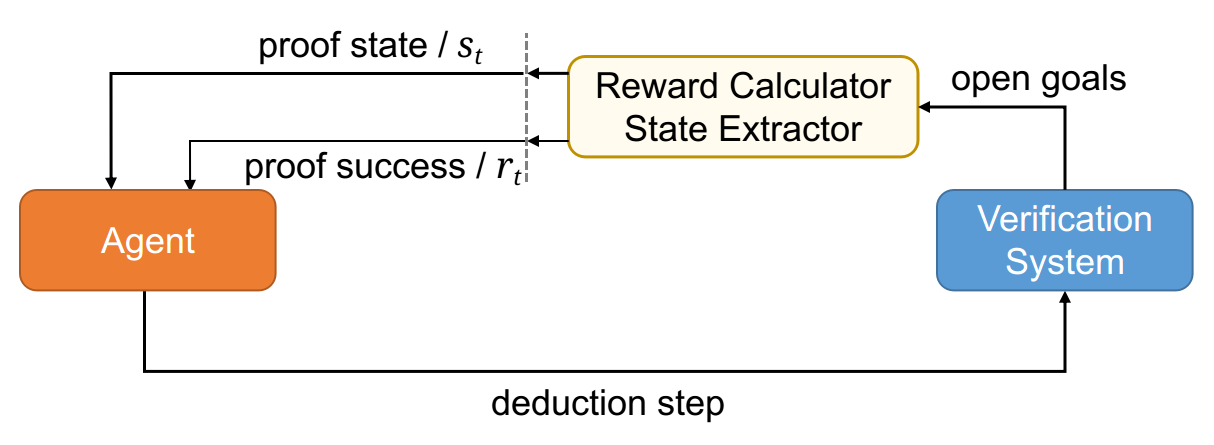
\includegraphics[width=0.8\textwidth]{img/rl4sv_schematic.png}
	\caption{An overview of the interplay between a rule-based program verifier and a deep RL system.}
	\label{f:rl4sv}
\end{figure}

\subsection*{Non-Linearity / Episodes and Goals}

It is not trivial to map the RL episode term to a process in the area of deductive rule-based verification. That is because the action flow of a single episode is inherently non-linear, but rather tree-like as there exist rule applications that may split a formula into multiple ones (see fig. \ref{f:ep}).

\begin{figure}[ht]
	\centering
	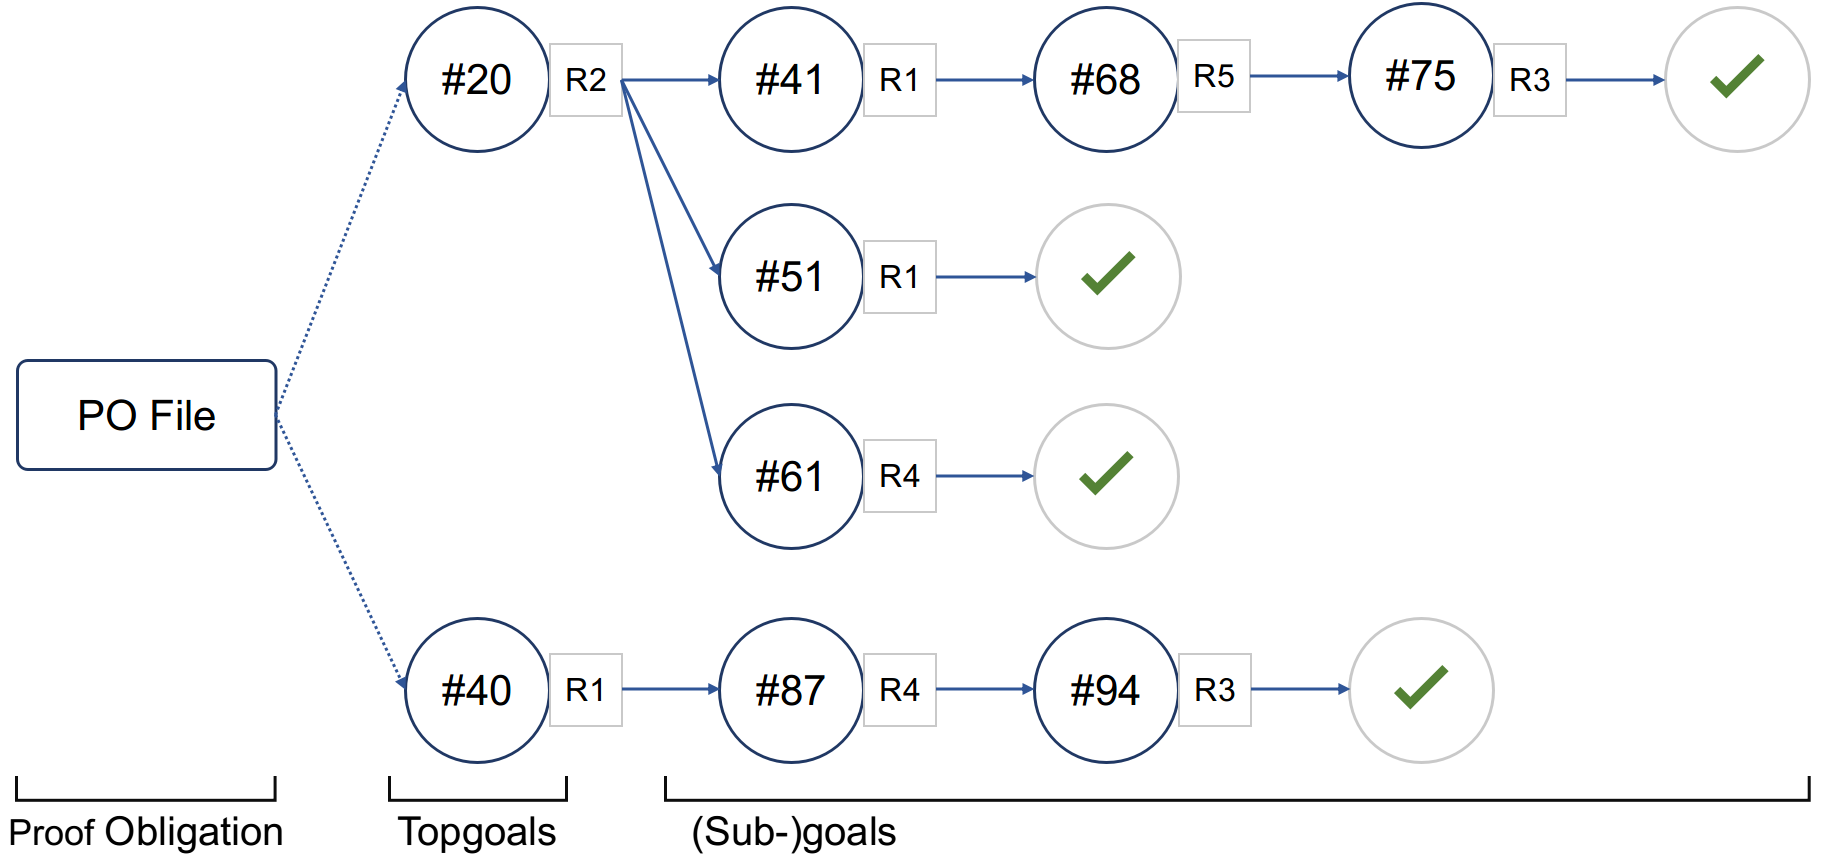
\includegraphics[width=0.8\textwidth]{img/rl_episode.png}
	\caption{An example episode of deductive rule-based verification. R1-R5 denote applications of different rules.}
	\label{f:ep}
\end{figure}

In deductive program verification a specification results in multiple \textit{proof obligations} (POs) which have to be proved in order to verify the specification. Every PO in turn consists of one or more sequents which have to be closed. The sequents are denoted as \textit{goals}, and the initially open goals are denoted as \textit{topgoals}. In fig. \ref{f:ep}, the goals are identified by a unique number.

Goals that are split as a result of a deduction step become \textit{parents}, and the resulting formulas become its \textit{children}. If a goal has become a parent, it is considered successfully closed only if all children have been successfully closed; otherwise it is considered failed. Furthermore, all goals that are not topgoals stem from previously handled goals and are therefore denoted as \textit{subgoals}. 

\subsection*{Episode Bounds}

First-order logic (the material our formulas are made of) in general is not decidable. This means that it is not possible to guarantee that every PO can be proved in a finite number of steps. For practical reasons, we hence assume that every PO that can be proved at all can be proved in a bounded and computationally feasible number of deduction steps.

An upper limit for deduction steps is imposed on each PO and the maximum depth of the proving tree of a topgoal is limited. We disregard every proof that exceeds these imposed limits, which means that we are learning the ability to practically prove POs instead of learning to determine the validity of them. As a consequence, verification episodes are finite.

If the limit of total deduction steps per PO is reached, the verification attempt of the whole PO is considered failed. Likewise, if the proof tree depth for a topgoal is reached, the proof attempt for the current topgoal is considered failed. If any goal proving attempt failed during an episode, e.g. though reaching these imposed proof size limits, the proof attempt of the whole PO is aborted and the episode ends.

\subsection*{Rewarding Scheme}

A rewarding scheme for rule-based verification, in our opinion, should satisfy three aspects: It should encourage a successful closing of topgoals, it should discourage the failure to close topgoals and it should encourage to find shorter paths for goal closure. Moreover, it is the domain experts' opinion that splits should be encouraged to happen only if all resulting children can be closed. If any child of a split goal fails to be closed, the split is penalized.

In order to better handle splits and their effects on the proof status, we introduce the term \textit{subepisode}: A subepisode is a segment of a proving tree starting from a topgoal or a goal directly resulting from a split, all containing all this goal's subgoals until closed or split again. In case of a split, each child marks the start of a new subepisode. In fig. \ref{f:ep}, for example, the opening of goal \#41 marks the start of a subepisode that ends with the closing of goal \#75.

\begin{table}[ht]
	\begin{tabularx}{\textwidth}{ |c|X| } \hline
		Name & Explanation \\ \hline \hline
		
		\texttt{open} & The newest goal is open and steps can still be made. \\ \hline
		\texttt{success} & The newest goal (and thus the subepisode) has been closed successfully. \\ \hline
		\texttt{fail} & The newest goal is open and steps cannot be made anymore (e.g. proof size/tree depth limit reached).\\ \hline
		\texttt{crash} & The verification system crashed or timed out. \\ \hline
		\texttt{parent} & The goal split into multiple subgoals. \\ \hline
		
	\end{tabularx}
\vspace*{2pt}
\caption{Statuses for subepisodes.}
\label{t:statuses}
\end{table}

Using the notion of subepisodes, the status of an episode is determined through the subepisodes it creates along the way. In order to retrieve the status for steps that split the currently open goal of a subepisode \texttt{e}, the resulting child goals and their respective subepisodes are worked through before assigning the status to the splitting step in \texttt{e}, as all children need to terminate successfully to propagate their success to the parent.

\subsection*{Training and Test Data}

In order to train effectively, the agent must be fed realistic data. For the domain of rule-based program verification, this would be formulas from the domain of first-order logic, stemming from a given set of specified programs. A set of 268 specification files has been prepared for a direct pick-up by the automatic mode of Ke\kern-.1em{Y}, containing 1322 topgoals. Their file paths are put into different text files in the folder \texttt{data/po\_files}, each containing a certain set of files.

\subsection*{Features}

When presented with a logical formula, it is the authors opinion that the best verification step to be applied can be derived from just the semantics of the formula. A consideration of the state of the verifier or the rule application history thus is only necessary if the rule/step is chosen by trial-and-error or if there is human uncertainty about the effects of applications or the verifier's configuration. As a result, a learned agent controller should be able to make informed decisions with just a representation of the current formula.

Within the scope Ke\kern-.1em{Y}, the formula of a goal is handled as an AST (see fig. \ref{f:ast}) where a node represents a symbol like a function, a quantifier or a constant, and its children represent its parameters or the symbols bound to it. Constants, numbers and similar symbols are represented as leaf nodes, as they don't bind any symbols to themselves. The root node of the AST is the implication linking antecedent and succedent, which in turn are modeled by a junction of one or more formulas or spared out if containing no formulas.

\begin{figure}[!htb]
	\centering
	{\Large$(\forall x: f(f(x)) = f(x)) \Rightarrow f(f(f(c))) = f(c)$}
	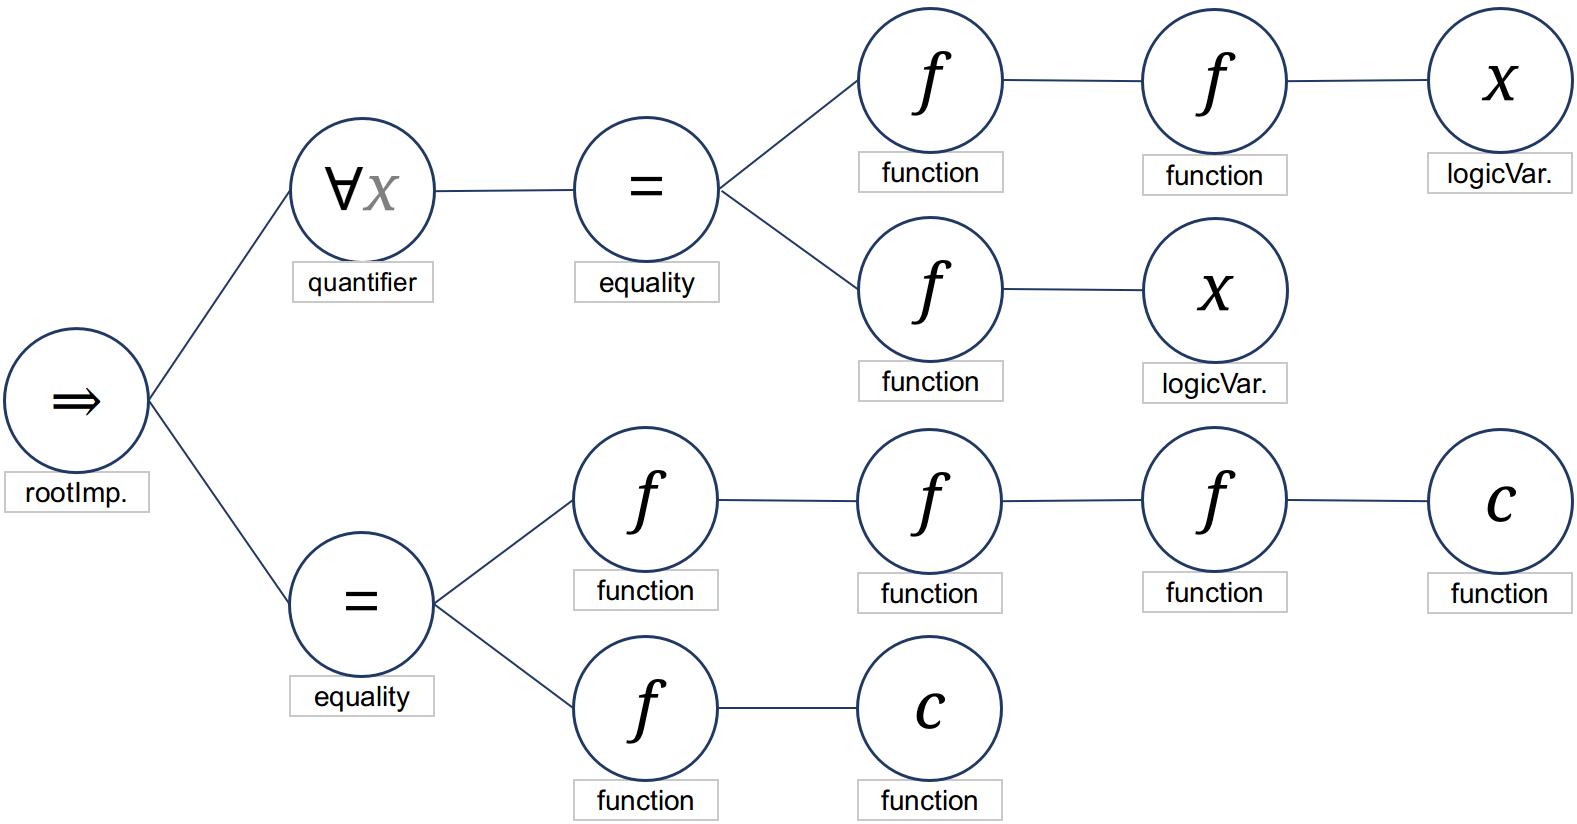
\includegraphics[width=0.8\textwidth]{img/goal_ast.png}
	\caption{An example formula and its AST.}
	\label{f:ast}
\end{figure}

When designing features for these formula AST, part of the semantics is extractable from the general shape of the AST and from the occurrences of certain symbols or symbol combinations. While domain knowledge is needed to determine which symbol categories are relevant and which are not, the features elicited for these categories are held as generic as possible, since the algorithm might discover regularities previously hidden from the domain experts. See table \ref{t:categories} for the categories considered and table \ref{t:features} for the complete list of features that are extracted from the formula ASTs.

\begin{table}[!htb]
	\begin{tabularx}{\textwidth}{ |c|X| } \hline
		Name & Contains \\ \hline \hline
		
		\textbf{\textit{equality}} & equality operator: \texttt{=} \\ \hline
		\textbf{\textit{inequality}} & inequality operators: \texttt{<}, \texttt{>},\texttt{<=},\texttt{>=} \\ \hline
		\textbf{\textit{heap}} & any symbol containing \texttt{heap} in its name \\ \hline
		\textbf{\textit{anonymity}} & any symbol containing \texttt{anon} in its name \\ \hline
		\textbf{\textit{numbers}} & the function with the name \texttt{Z}, which identifies numbers \\ \hline
		\textbf{\textit{programConstants}} & any symbol of the class \textit{programConstants} \\ \hline
		\textbf{\textit{modalities}} & any symbol of the class \textit{modalities} \\ \hline
		\textbf{\textit{ITE}} & the symbols \texttt{IfThenElse} and \texttt{IfExThenElse} \\ \hline
		\textbf{\textit{depContracts}} & any symbol of the classes \textit{ProgramMethod} and \textit{ObersverFunction} \\ \hline
		\textbf{\textit{quantifiers}} & the quantifiers $\forall$ and $\exists$ \\ \hline
	\end{tabularx}
\vspace*{2pt}
\caption{The predetermined feature categories and which symbol occurrences are included in them.}
\label{t:categories}
\end{table}

\begin{table}[!htb]
	\begin{tabularx}{\textwidth}{ |c|X|c|c| } \hline
		Feature $f$ & Explanation & $\mu_f$ & $\sigma_f$ \\ \hline \hline
			
		\textbf{\textit{astSize}} 		
		& The number of nodes of an AST.
		& $314.483$ & $324.699$ \\ \hline
		\textbf{\textit{astHeight}}		
		& A relative AST height measure that uses the cumulated depth of all nodes: -1 indicates the widest possible tree, +1 the tallest possible tree.
		& $-0.876$ & $0.089$ \\ \hline
		\textbf{\textit{formulaCount}}	
		& The number of formulas the antecedent and succedent hold.
		& $16.925$ & $12.137$ \\ \hline
		\textbf{\textit{selectStoreCnt}}	
		& The number of occurrences of the combined \texttt{select(store())} function.
		& $0.135$ & $1.368$ \\ \hline \hline
			
		\textbf{\textit{isPresent}} 		
		& +1 if symbols of a category are present in this AST, -1 otherwise.
		& - & - \\ \hline
		\textbf{\textit{balance}} 		
		& Smaller if the occurrences of a category are found more to the left side of the AST, bigger if found more to the right side. Ranges from -1 to +1.
		& - & - \\ \hline
		\textbf{\textit{spread}} 		
		& Smaller if occurrences of a category are found concentrated in a single spot, bigger if they are more spread out. Ranges from -1 to +1.
		& - & - \\ \hline
		\textbf{\textit{relCount}} 		
		& Number of category occurrences divided by total symbol count.
		& $< 0.103$ & $< 0.059$ \\ \hline
		\textbf{\textit{relDepth}} 		
		& Average depth of category occurrences divided by average depth of all symbols.
		& $< 0.667$ & $< 0.133$ \\ \hline
	\end{tabularx}
\vspace*{2pt}
\caption{The features elicited, their explanations and distribution information for non-normalized features. The upper half contains the general AST features while the lower half contains the per-category features.}
\label{t:features}
\end{table}

All in all, a total of 54 features is observed. Because they differ in their definition range and characteristic values, a normalization process is undertaken for every feature but the \textit{present}, the \textit{spread} and the \textit{balance} feature: Using each feature $f$'s values $x_f$ for all topgoals in the available data set, the feature's mean $\mu_f$ and standard deviation $\sigma_f$ are computed. When extracting features for the learning or usage process afterwards, these figures are fed into a feature-specific tanh function: 

\begin{equation}
x'_{f} = tanh(\frac{x_f-\mu_f}{2\sigma_f})
\end{equation}

As a result, the normalized values $x'_f$ of every feature $f$ range from -1 to 1, which might optimize the numerical stability of underlying deep learning policies.


\subsection*{Actions: Tactics}
\label{ss:tac}

In Ke\kern-.1em{Y}, the whole set of applicable rules consists of over 1000 different deduction rules. Hence, for the sake of simplicity, we introduced the concept of \textit{tactics} to Ke\kern-.1em{Y}. A tactic is a collection of deduction rules for simplification and reshaping, also including a procedure description on how to apply this set of rules on a formula. This means that the selection of a tactic also applies the included rules according to given description. Tactics are manually created, each covering a certain area or theory of the underlying formula logic or behaving in a distinctive way (see table \ref{t:tactics}). The tactics \textbf{\textit{INT}}, \textbf{\textit{HEAP}} and \textbf{\textit{EQUALITY}} are specialized subsets of \textbf{\textit{AUTO}}, which means that \textbf{\textit{AUTO}} can do everything the other three tactics can. Albeit, it works at a considerably slower pace.

\begin{table}[ht]
	\begin{tabularx}{\textwidth}{ |c|X| } \hline
		Name & Explanation \\ \hline \hline
		
		\textbf{\textit{AUTO}} & Mimics the automatic strategy currently used by  Ke\kern-.1em{Y}. \\ \hline
		\textbf{\textit{AUTO\_NOSPLIT}} & Same as \textbf{\textit{AUTO}} but avoids goal splits. \\ \hline
		\textbf{\textit{SMT}} & Outsources the current goal to an SMT solver. \\ \hline
		\textbf{\textit{MODELSEARCH}} & Tries to find variable instantiations that satisfy the goal. \\ \hline
		\textbf{\textit{DEPENDENCY}} & Tries to resolve program dependencies present in the goal. \\ \hline
		\textbf{\textit{EXPAND}} & Expands a function definition. \\ \hline
		\textbf{\textit{QUANT}} & Instantiates quantors found in the goal. \\ \hline
		\textbf{\textit{HEAP}} & Subset of \textbf{\textit{AUTO}}'s rules, focusing on memory allocation and usage statements. \\ \hline
		\textbf{\textit{INT}} & Subset of \textbf{\textit{AUTO}}'s rules, focusing on integer arithmetic. \\ \hline
		\textbf{\textit{EQUALITY}} & Subset of \textbf{\textit{AUTO}}'s rules, focusing on equalities. \\ \hline
	\end{tabularx}
\vspace*{2pt}
\caption{Tactics implemented in Ke\kern-.1em{Y}.}
\label{t:tactics}
\end{table}

The verification process using tactics is analogous to using singular rules, in that selecting a tactic can produce new goals and depth-first search is employed until no more goals are open. Likewise, tactic selections which have no effect leave the currently active goal as-is.

% ==================================================================================================

\section*{Related Work}
\label{ss:rw}

\subsection*{ML for Methods of Formal Verification}

Due to the complexity of the problem domain, the application of ML to FV has only picked up pace in the last few years, although first attempts have already been made decades ago \cite{lounisIntegratingMachinelearningTechniques1993}.

In the survey paper of Amrani et al. (2018), a general insight is given into the impact of ML techniques when applied to various fields within the FV domain \cite{amraniMLFVSurvey2018a}. According to the authors, areas in which ML has brought improvements include SAT/SMT solving (e.g. \cite{DBLP:conf/aaai/SamulowitzM07}, \cite{hutterPerformancePredictionAutomated2006} and \cite{wuImprovingSATsolvingMachine2017}), Theorem Proving (e.g \cite{bridgeMachineLearningFirstOrder2014}, \cite{kuhlweinMaLeSFrameworkAutomatic2015} and \cite{kuhlweinOverviewEvaluationPremise2012}), Model Checking (e.g. \cite{DBLP:conf/mochart/AraragiC06}, \cite{clarkeSATBasedAbstractionRefinement2002}) and Static Analysis (e.g. \cite{yerimaAndroidMalwareDetection2014},\cite{kimClassifyingSoftwareChanges2008}).

The area of Software Verification is most similar to Amrani's area of Theorem Proving, dealing with the (dis-)proving of software/system semantics which have been expressed in mathematical theories. For some SV tools (included in the comprehensive participants list of the \textbf{VerifyThis} challenge \cite{ernstVerifyThisVerificationCompetition2019}) there exist augmentation approaches which use ML:

For the Isabelle proof assistant \cite{technischeuniversitatmunchenIsabelle}, Blanchette et al. have presented a new theorem selector that uses the Sparse Naive Bayes and k-Nearest Neighbors algorithms to select a suitable subset of all usable theorems. \cite{blanchetteLearningBasedFactSelector2016}.

For Why3 \cite{filliatreWhy3WherePrograms2013}, a program verification tool outsourcing the proving of theorems to a variety of automated Theorem Provers, the Where4 extension estimates runtime figures using regression and chooses the ATP with the best runtime prediction \cite{healyPredictingSMTSolver2017}.

For the higher-order logic prover Satallax \cite{brownSatallaxAutomaticHigherOrder2012}, Färber and Brown introduced a proof guidance method adjusting the delay with which propositions are processed, based on the classification result of a naive-bayes classifier \cite{farberInternalGuidanceSatallax2016}.

\subsection*{Deep Reinforcement Learning}

RL, especially with the fusion of deep learning methods, has been credited for a large part of the recent advances in Artificial Intelligence. Its application improved the state of the art in domains such as generating text (\cite{guoGeneratingTextDeep2015}), playing (video) games (\cite{ohActionConditionalVideoPrediction2015}, \cite{silverMasteringGameGo2017}) or navigating robots (\cite{kahnSelfSupervisedDeepReinforcement2018a}).

Perhaps most similar to our domain is the work of Crouse et al. \cite{crouseDeepReinforcementLearning2020}. There, RL is used for internal guidance in a rule-based reasoning process: the agent decides at each step which inference rule to apply to a clause.

The results indicate that the performance of such a neural network trained with RL is comparable to existing reasoners, although slightly worse than the reasoner is was compared with (which is Beagle \cite{baumgartnerBeagleHierarchicSuperposition2015}).

% ==================================================================================================

%\newpage
% \section{Bibliography}
% \label{s:bib}
% ------------------

\bibliographystyle{splncs04}
\bibliography{gym-autokey_explanation}

\end{document}